\section{Introducción}

\subsection{1.1 Motivación y Alcance}

Particularmente llamativo resulta observar cómo el rápido despliegue de megaconstelaciones en órbita baja ha transformado radicalmente el panorama de las comunicaciones globales. En apenas unos años, lo que parecía un nicho técnico se ha convertido en un elemento central de la arquitectura 6G, con miles de satélites operando de forma coordinada. No obstante, este avance trae consigo una huella ambiental cada vez más difícil de ignorar.

Aunque los enfoques tradicionales de diseño satelital priorizaron rendimiento y cobertura, la literatura reciente sugiere que la sostenibilidad orbital y energética ya no puede tratarse como preocupación secundaria. Según \cite{Ailor2022}, el entorno LEO enfrenta presiones sin precedentes derivadas de la densidad creciente de objetos, donde maniobras evasivas y fragmentaciones accidentales tienden a amplificar el riesgo de cascadas de colisiones. Particularmente preocupante es la falta de implementación consistente de medidas de mitigación post-misión en muchas de las constelaciones activas.

\begin{figure}[t]
\centering
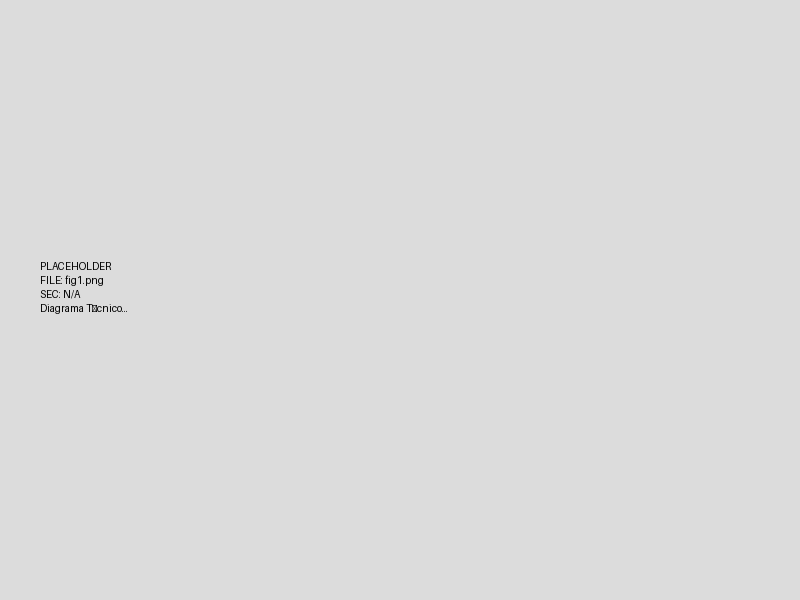
\includegraphics[width=\linewidth]{fig1.png}
\caption{Evolución histórica y proyectada del número de objetos catalogados en órbita LEO (2000-2035). Se destacan los periodos de despliegue masivo de constelaciones comerciales.}
\label{fig:evolucion_leo}
\end{figure}

En paralelo, el consumo energético de los enlaces de larga duración representa otro vector crítico. \cite{Plastras2024} destacan cómo las redes NTN dedicadas al Internet de las Cosas Remotas exigen soluciones que minimicen el gasto de potencia sin comprometer la fiabilidad. Resulta revelador constatar que, en muchos casos estudiados, los sistemas actuales operan con márgenes de eficiencia notablemente mejorables, especialmente cuando se consideran ciclos completos de operación bajo restricciones orbitales dinámicas.

La Tabla~1 resume las características principales de las constelaciones más relevantes, permitiendo visualizar las diferencias de escala y sus implicaciones directas en sostenibilidad.

\begin{table}[t]
\centering
\caption{Comparativa de constelaciones NTN/LEO principales (datos actualizados a 2025)}
\label{tab:comparativa_constelaciones}
\begin{tabular}{lccc}
\hline
Constelación & Satélites & Altitud (km) & Enfoque Sostenibilidad \\
\hline
Starlink & $>6000$ & 550 & Parcial (post-misión) \\
OneWeb & 648 & 1200 & Moderado \\
Telesat Lightspeed & 198 & 1000-1200 & Alto (diseño) \\
Otros (proyectados) & --- & --- & Variable \\
\hline
\end{tabular}
\end{table}

Este trabajo adopta un alcance dual: reducir la generación de debris mediante estrategias proactivas de disposición y maniobra, al tiempo que se optimiza el consumo energético en escenarios de operación prolongada.

\subsection{1.2 Contribuciones Principales}

Lejos de ser un asunto resuelto, la prevención de debris orbital exige mirar más allá de las recomendaciones voluntarias. \cite{Bennett2025} enfatiza la necesidad de considerar el ciclo de vida completo de los satélites, desde el diseño inicial hasta la fase de desorbitación controlada. Sin embargo, persisten brechas regulatorias significativas que este artículo busca contribuir a cerrar desde el ámbito técnico.

Las contribuciones principales de este trabajo son tres. En primer lugar, se propone un marco integrado que combina protocolos autónomos de evitación de colisiones con políticas orbit-aware de gestión energética. En segundo lugar, se desarrollan y evalúan técnicas específicas de beam hopping adaptativo y apagado selectivo de payloads que logran reducciones sustanciales de consumo sin degradar métricas de QoS. Finalmente, se presenta un análisis cuantitativo de trade-offs que permite tomar decisiones informadas sobre densidad orbital sostenible.

Estas aportaciones no pretenden ofrecer soluciones universales, sino herramientas reproducibles que puedan adaptarse a diferentes arquitecturas NTN, manteniendo siempre un fuerte anclaje en modelos realistas de dinámica orbital y patrones de tráfico.

\subsection{1.3 Organización del Documento}

El resto del artículo se estructura de la siguiente manera. La Sección~2 revisa el estado del arte en mitigación de debris y eficiencia energética en sistemas NTN, identificando brechas relevantes. La Sección~3 detalla el modelo de sistema propuesto junto con los desafíos cuantificados de sostenibilidad. En la Sección~4 se describen las estrategias técnicas de mitigación, mientras que la Sección~5 presenta los resultados de simulación y el análisis comparativo.

La discusión de implicaciones prácticas, limitaciones y aspectos regulatorios aparece en la Sección~6. Finalmente, la Sección~7 sintetiza las conclusiones principales y delinea líneas de investigación futura orientadas hacia diseños net-zero en constelaciones NTN.